

\begin{frame}{3 steps in constructing a tree}
    \begin{center}
        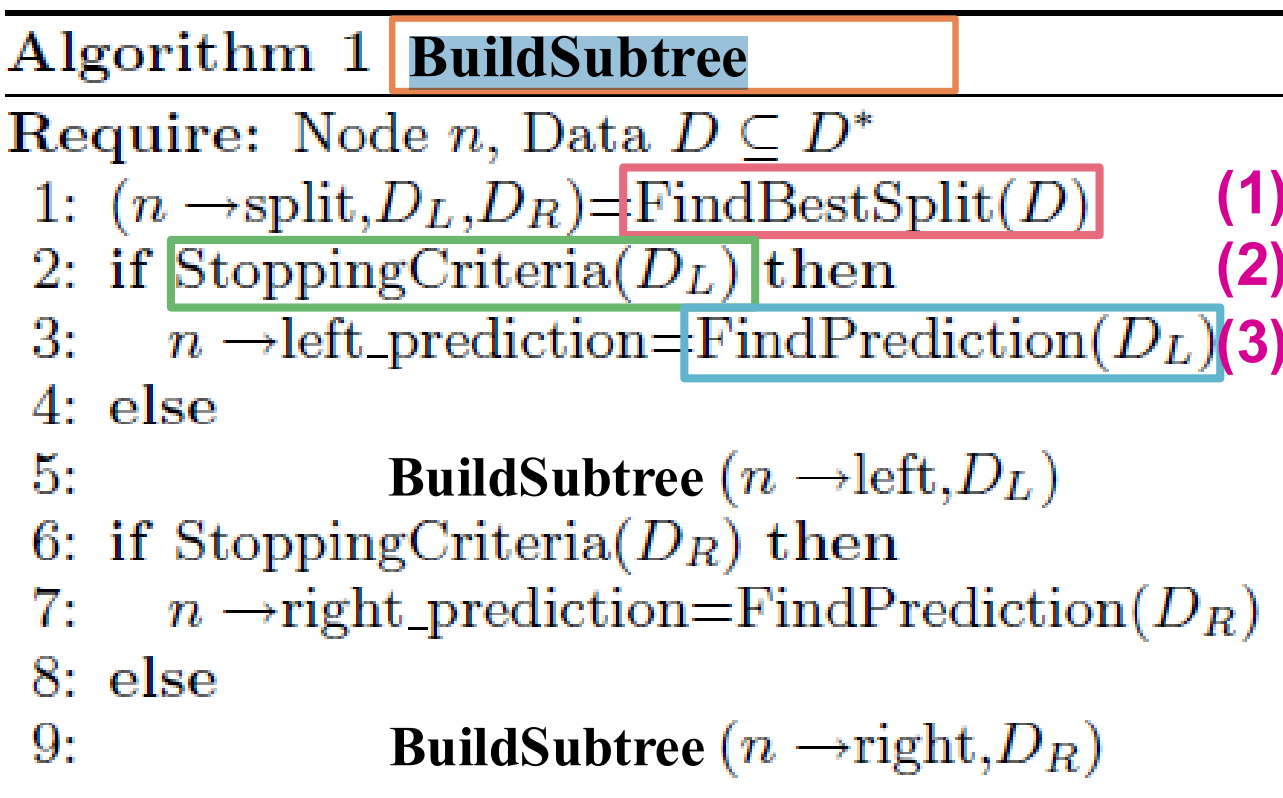
\includegraphics[width=0.85\linewidth]{images/decision-trees/decision-trees-9.png}
    \end{center}

    \vspace{0.3cm}
    \begin{itemize}
        \item Requires at least a single pass over the data!
    \end{itemize}
\end{frame}


\begin{frame}{How to construct a tree?}
    \begin{columns}
        \begin{column}{0.75\textwidth}
            \begin{itemize}
                \item (1) How to split? Pick attribute \& value that optimizes some criterion
                \item Regression: Purity
                \begin{itemize}
                    \item Find split $(X^{(i)}, v)$ that creates $D, D_L, D_R$: parent, left, right child datasets and maximizes:
                    \[
                    |D| \cdot Var(D) - (|D_L| \cdot Var(D_L) + |D_R| \cdot Var(D_R))
                    \]
                    \item $Var(D) = \frac{1}{|D|} \sum_{i \in D} (y_i - \bar{y})^2$ \quad ... variance of $y_i$ in $D$
                \end{itemize}
            \end{itemize}
        \end{column}
        \begin{column}{0.25\textwidth}
            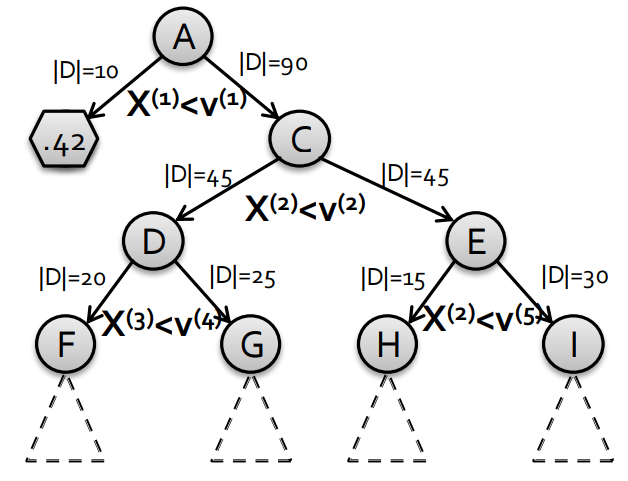
\includegraphics[width=\linewidth]{images/decision-trees/decision-trees-10.png}
        \end{column}
    \end{columns}
\end{frame}


\begin{frame}{How to construct a tree?}
    \begin{columns}
        \begin{column}{0.65\textwidth}
            \begin{itemize}
                \item (1) How to split? Pick attribute \& value that optimizes some criterion
                \item Classification: Information Gain
                \begin{itemize}
                    \item Measures how much a given attribute $X$ tells us about the class $Y$
                    \item $IG(Y \mid X)$: We must transmit $Y$ over a binary link. How many bits on average would it save us if both ends of the line knew $X$?
                \end{itemize}
            \end{itemize}
        \end{column}
        \begin{column}{0.35\textwidth}
            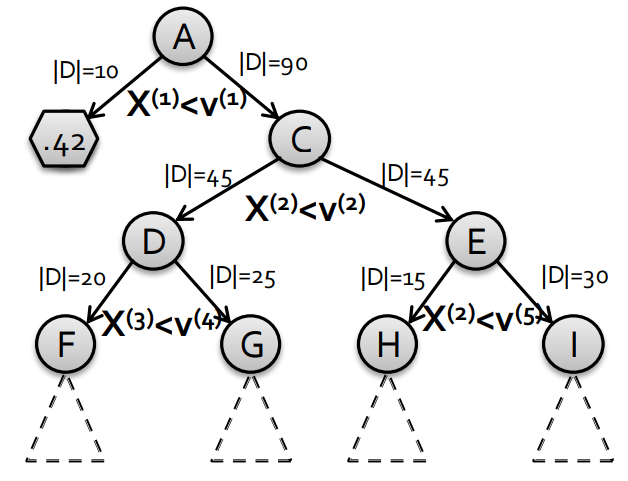
\includegraphics[width=\linewidth]{images/decision-trees/decision-trees-10.png}
        \end{column}
    \end{columns}
\end{frame}

\begin{frame}{Why Information Gain? Entropy}

\textbf{The entropy of} $X$: \\
\[
H(X) = - \sum_{j=1}^{m} p(X_j) \log p(X_j)
\]

\begin{itemize}
  \item ``High Entropy": $X$ is from a uniform (boring) distribution
  \begin{itemize}
    \item A histogram of the frequency distribution of values of $X$ is \textbf{flat}
  \end{itemize}

  \item ``Low Entropy": $X$ is from a varied (peaks/valleys) distribution
  \begin{itemize}
    \item A histogram of the frequency distribution of values of $X$ would have many lows and one or two highs
  \end{itemize}
\end{itemize}

\begin{center}
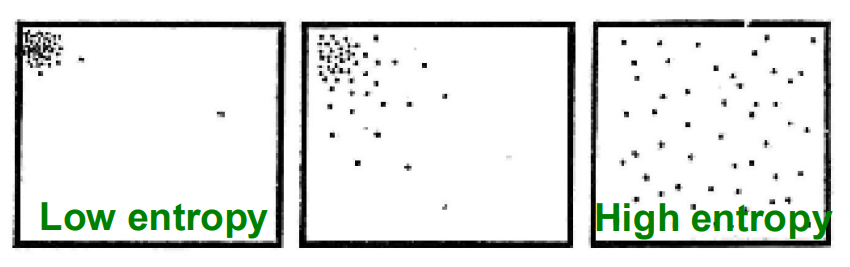
\includegraphics[width=0.65\textwidth]{images/decision-trees/decision-trees-11.png}
\end{center}

\end{frame}


\begin{frame}[allowframebreaks]{Why Information Gain? Entropy}

\begin{itemize}
  \item Suppose I want to predict $Y$ and I have input $X$
  \begin{itemize}
    \item $X$ = College Major
    \item $Y$ = Likes “Casablanca”
  \end{itemize}
\end{itemize}

\begin{center}
\begin{tabular}{|c|c|}
\hline
X & Y \\
\hline
Math & Yes \\
History & No \\
CS & Yes \\
Math & No \\
Math & No \\
CS & Yes \\
Math & Yes \\
History & No \\
\hline
\end{tabular}
\end{center}

\begin{itemize}
  \item From this data we estimate
  \begin{itemize}
    \item $P(Y = Yes) = 0.5$
    \item $P(X = Math \land Y = No) = 0.25$
    \item $P(X = Math) = 0.5$
    \item $P(Y = Yes \mid X = History) = 0$
  \end{itemize}
  \item Note:
  \begin{itemize}
    \item $H(Y) = -\frac{1}{2} \log_2(\frac{1}{2}) - \frac{1}{2} \log_2(\frac{1}{2}) = 1$
    \item $H(X) = 1.5$
  \end{itemize}
\end{itemize}

\end{frame}


\begin{frame}[allowframebreaks]{Why Information Gain? Entropy}

\begin{itemize}
  \item Suppose I want to predict $Y$ and I have input $X$
  \begin{itemize}
    \item $X$ = College Major
    \item $Y$ = Likes ``Casablanca''
  \end{itemize}
\end{itemize}


\begin{itemize}
  \item Def: Specific Conditional Entropy
  \begin{itemize}
    \item $H(Y \mid X = v)$ = The entropy of $Y$ among only those records in which $X$ has value $v$
  \end{itemize}
  \item Example:
  \begin{itemize}
    \item $H(Y \mid X = Math) = 1$
    \item $H(Y \mid X = History) = 0$
    \item $H(Y \mid X = CS) = 0$
  \end{itemize}
\end{itemize}

\end{frame}


\begin{frame}[allowframebreaks]{Why Information Gain?}

\begin{itemize}
  \item Suppose I want to predict $Y$ and I have input $X$
  \begin{itemize}
    \item $X$ = College Major
    \item $Y$ = Likes ``Casablanca''
  \end{itemize}
\end{itemize}


\begin{itemize}
  \item Def: Conditional Entropy
  \begin{itemize}
    \item $H(Y \mid X)$ = The average specific conditional entropy of $Y$
    \item = the entropy of $Y$, conditioned on $X$, if you choose a record at random
    \item $= \sum_j P(X = v_j) H(Y \mid X = v_j)$
  \end{itemize}
\end{itemize}

\end{frame}



\begin{frame}[allowframebreaks]{Why Information Gain?}

\begin{itemize}
  \item Suppose I want to predict $Y$ and I have input $X$
  \begin{itemize}
    \item $X$ = College Major
    \item $Y$ = Likes ``Casablanca''
  \end{itemize}
\end{itemize}


\begin{itemize}
  \item $H(Y \mid X)$ = The average specific conditional entropy of $Y$
  \[
  = \sum_j P(X = v_j) H(Y \mid X = v_j)
  \]
  \item Example:
\end{itemize}

\begin{center}
\begin{tabular}{|c|c|c|}
\hline
$v_j$ & $P(X = v_j)$ & $H(Y \mid X = v_j)$ \\
\hline
Math & 0.5 & 1 \\
History & 0.25 & 0 \\
CS & 0.25 & 0 \\
\hline
\end{tabular}
\end{center}

\begin{itemize}
  \item So: $H(Y \mid X) = 0.5 \cdot 1 + 0.25 \cdot 0 + 0.25 \cdot 0 = 0.5$
\end{itemize}

\end{frame}


\begin{frame}[allowframebreaks]{Why Information Gain?}

\begin{itemize}
  \item Suppose I want to predict $Y$ and I have input $X$
  \begin{itemize}
    \item $X$ = College Major
    \item $Y$ = Likes ``Casablanca''
  \end{itemize}

  \item Def: Information Gain
  \begin{itemize}
    \item $IG(Y \mid X)$ = I must predict $Y$. How much information do I get about $Y$ if I knew $X$?
    \[
    IG(Y \mid X) = H(Y) - H(Y \mid X)
    \]
  \end{itemize}
  
  \item Example:
  \begin{itemize}
    \item $H(Y) = 1$
    \item $H(Y \mid X) = 0.5$
    \item Thus $IG(Y \mid X) = 1 - 0.5 = 0.5$
  \end{itemize}
\end{itemize}


\end{frame}


\begin{frame}[allowframebreaks]{What is Information Gain used for?}

\begin{itemize}
  \item Suppose you are trying to predict whether someone is going to live past 80 years

  \item From historical data you might find:
  \begin{itemize}
    \item $IG(LongLife \mid HairColor) = 0.01$
    \item $IG(LongLife \mid Smoker) = 0.4$
    \item $IG(LongLife \mid Gender) = 0.25$
    \item $IG(LongLife \mid LastDigitOfSSN) = 0.00001$
  \end{itemize}

  \item IG tells us how much information about $Y$ is contained in $X$
  \begin{itemize}
    \item So attribute $X$ that has high $IG(Y \mid X)$ is a good split!
  \end{itemize}
\end{itemize}

\end{frame}


\begin{frame}[allowframebreaks]{3 steps in constructing a tree}
    \begin{center}
        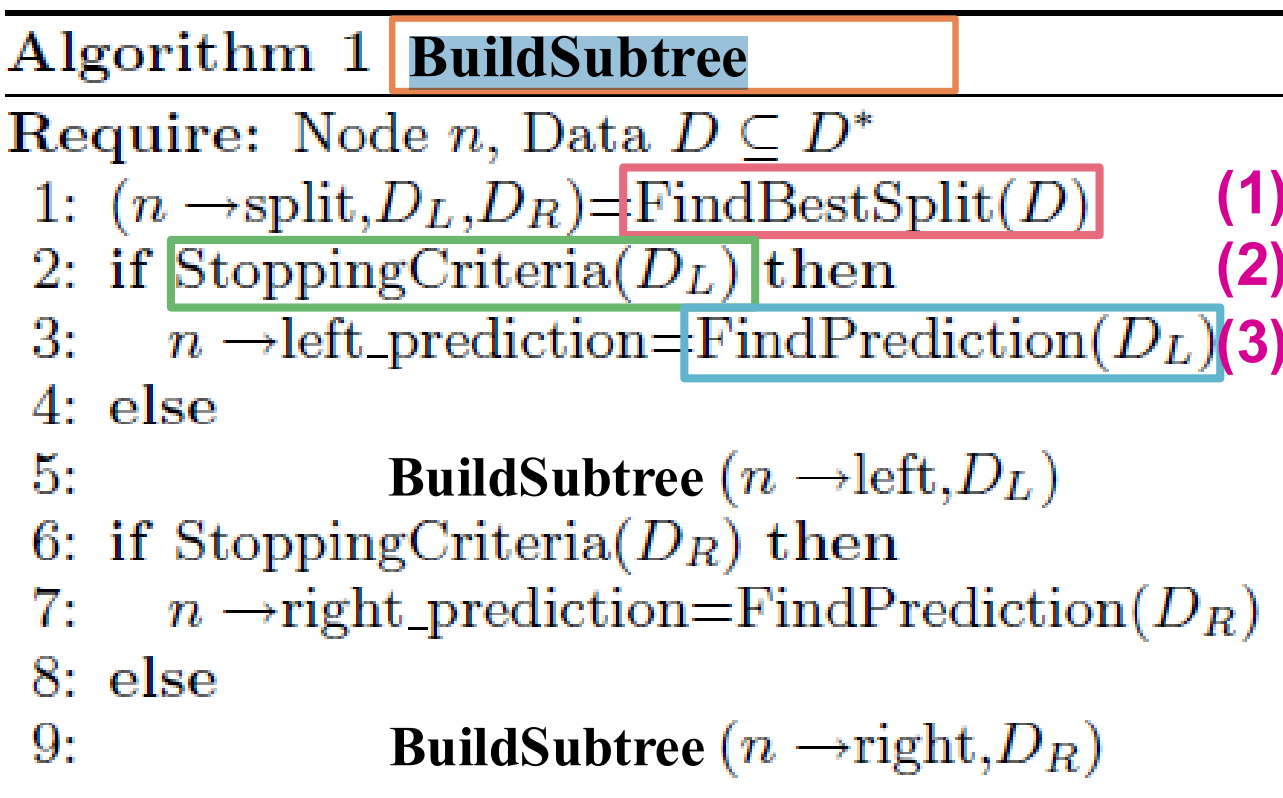
\includegraphics[width=0.9\linewidth]{images/decision-trees/decision-trees-9.png}
    \end{center}
\end{frame}

\begin{frame}[allowframebreaks]{When to stop?}
    \begin{columns}
        \begin{column}{0.6\textwidth}
            \begin{itemize}
                \item \textbf{(2) When to stop?}
                \item Many different heuristic options
                \item \textbf{Two ideas:}
                \begin{itemize}
                    \item (1) When the leaf is ``pure''
                    \begin{itemize}
                        \item The target variable does not vary too much: $Var(y) < \varepsilon$
                    \end{itemize}
                    \item (2) When \# of examples in the leaf is too small
                    \begin{itemize}
                        \item For example, $|D| \leq 100$
                    \end{itemize}
                \end{itemize}
            \end{itemize}
        \end{column}
        \begin{column}{0.4\textwidth}
            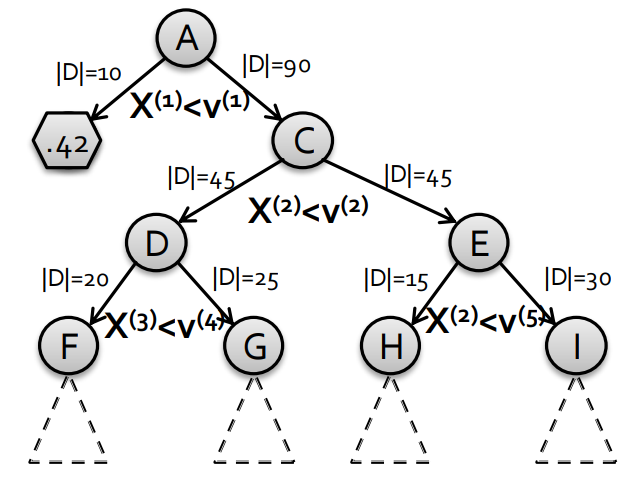
\includegraphics[width=\linewidth]{images/decision-trees/decision-trees-12.png}
        \end{column}
    \end{columns}
\end{frame}


\begin{frame}[allowframebreaks]{How to predict?}
    \begin{columns}
        \begin{column}{0.6\textwidth}
            \begin{itemize}
                \item \textbf{(3) How to predict?}
                \item \textbf{Many options}
                \begin{itemize}
                    \item \textbf{Regression:}
                    \begin{itemize}
                        \item Predict average $y_i$ of the examples in the leaf
                        \item Build a linear regression model on the examples in the leaf
                    \end{itemize}
                    \item \textbf{Classification:}
                    \begin{itemize}
                        \item Predict most common $y_i$ of the examples in the leaf
                    \end{itemize}
                \end{itemize}
            \end{itemize}
        \end{column}
        \begin{column}{0.4\textwidth}
            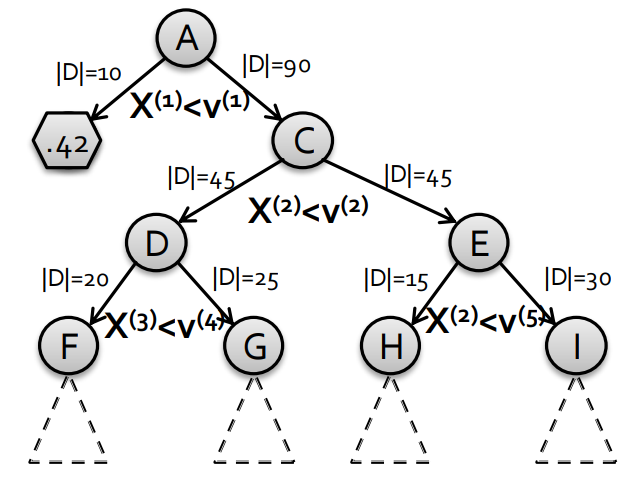
\includegraphics[width=\linewidth]{images/decision-trees/decision-trees-12.png}
        \end{column}
    \end{columns}
\end{frame}
